\documentclass[a4paper,12pt]{article}
\usepackage[UTF8]{ctex}
\usepackage{amsmath,amsthm,amssymb}
\usepackage{graphicx}
\usepackage{geometry}
\usepackage{array}
\usepackage{pgfplots}
\usepackage{pgfplotstable}
\usepackage{tikz}
\usepackage{multirow}
\usepackage{enumitem}
\pgfplotsset{compat=1.18}
\geometry{left=2cm, right=2cm, top=2cm, bottom=2cm}

\title{决策方法论期中复习}
\author{核31\kern 36pt 钱昊远\kern 12pt 整理}
\date{2024年11月2日}

\begin{document}

\maketitle

\section{基本知识}

\subsection{概率公式}

\noindent
\textbf{条件概率}

事件$B$在另外一个事件$A$已经发生条件下发生的概率。条件概率表示为$P(B\mid A)$。

条件概率有以下相关公式:
$$
P(B \mid A)= \frac{P(AB)}{P(A)}
$$
$$
P(AB)=P(A)P(B \mid A)
$$
$$
P(A_{1}A_{2}\cdots A_{n})=P(A_{1})P(A_{2} \mid A_{1})P(A_{3} \mid A_{1}A_{2})
\cdots P(A_{n} \mid A_{1}A_{2}A_{3}\cdots A_{n-1})
$$

\noindent
\textbf{全概率公式}

设$B_{1},B_{2},\dots ,B_{n}$是样本空间$\Omega$的一个分割,即$B_{i}$之间互不相容,
且$\cup _{i=1}^{n}B_{i}=\Omega$,若有$P(B_{i})>0$,则对于任意事件$A$有:
$$
P(A)=\sum_{i=1}^{n}P(B_{i})P(A \mid B_{i})
$$

\noindent
\textbf{贝叶斯公式}

$$
P(B_{i} \mid A)=\frac{P(AB_{i})}{P(A)}=\frac{P(B_{i})P(A \mid B_{i})}{\sum P(B_{j})P(A \mid B_{j})}
$$

\subsection{决策问题}

\noindent
\textbf{决策分析过程的概念}

决策分析过程是:
人们为了实现某一特定目标,在占有一定信息和经验的基础上,根据主客观条件的可能性,提出各种可行方案;
之后采用一定的科学方法和手段,进行比较、分析和评价,按照决策准则,从中筛选出最满意的方案;
并根据方案实施的反馈情况,对方案进行修正调整,直至目标实现的整个系统过程。

\noindent
\textbf{决策基本要素}

决策者(Decision Maker):
决策的主题,可以是个体,也可以是群体。

决策目标(Decision Objectives):
希望达到的明确的目标,可以是单个目标,也可以是多个目标。

备选方案(Decision Alternatives):
可供选择的不同的决策方案,可以是有限个明确的方案,也可能是无限多种可能。

自然状态(States of Nature):
决策者无法控制但可以预见的决策环境客观存在的各种状态,可以是确定,或者不确定的。

方案结果(Decision Outcomes):
各种决策方案在不同的自然状态下所出现的结果。

决策准则(Decision Criteria):
评价方案是否达到决策目标的价值标准,备选方案选择的依据。

\noindent
\textbf{决策问题的分类}

按照自然状态的种类来分类(对自然状态的了解程度从高到低):
确定型决策(Decision-Making Under Certainty)、风险型决策(Decision-Making Under Risk)、
不确定型决策(Decision-Making Under Uncertainty)
  
按照决策目标的多少来分类:单目标决策、多目标决策
  
按照决策过程的连续性分类:单项决策、序贯决策(多阶段)
  
按照方案结果量化程度分类:定性决策、定量决策
  

\section{单目标决策——确定型决策}

确定型决策是指只存在一种完全确定的自然状态的决策,存在一个明确的决策目标,且可求得各方案在确定自然状态下的损益值。
其决策目标通常是寻找达到最优解的备选方案,例如用有限的人力、物力、财力等资源取得最好的经济效果。
通常可使用运筹学方法进行求解分析,包括线性规划、非线性规划、动态规划、队列理论等方法。

\section{单目标决策——风险型决策}

\subsection{风险型决策的概念}

风险型决策,也称随机型决策,是决策者根据几种不同的自然状态可能的发生概率所进行的决策。

\subsection{风险型决策决策准则}

\noindent
\textbf{期望值准则}
 
设风险型决策问题有$m$种备选方案,$n$种自然状态,备选方案$a_{i}(i=1,2,\cdots,m)$的方案结果(损益值)为随机变量$C_{i}$,
其在自然状态$s_{j}(j=1,2,\cdots,n)$下的取值为$c_{ij}$ ,自然状态$j$出现的概率为$p_{j}$,则备选方案$i$的期望为:
$$
E(C_{i})=\sum_{j=1}^{n}p_{j}\cdot c_{ij}
$$
选择收益期望值最大或者损失期望值最小的方案为最优方案。

决策分析中定义的离差为:
$$
\sigma_{i}=E(C_{i})-\min_{j}(c_{ij})
$$
如果期望收益值最大(或期望损失值最小)的方案不止一个时,可以选取离差最小的方案为最优方案,即选取最差情况最优的方案。

\noindent
\textbf{最大可能性准则}

$A$为$m$种备选方案的集合$\left\{a_{1},a_{2},\cdots,a_{m}\right\}$,
$S$为$n$种自然状态的集合$\left\{s_{1},s_{2},\cdots,s_{m}\right\}$,
$P(s)$为状态$s$出现的概率,$s_{likely}$为出现概率最高的自然状态,
$C(a,s)$为备选方案$a$在自然状态$s$下的收益,$a^*$为最大可能性准则下选择的备选方案,则
$$
a^*=\text{arg}\max_{a\in A}C\left(a,s_{likely}\right)
$$
$$
s_{likely}=\text{arg}\max_{s\in S}P\left(s\right)
$$
即根据概率最大的自然状态进行决策。

\subsection{风险型决策中完整情报的价值}

通过调查分析,可以获取自然状态的完整情报,具有完整情报的最大期望收益为:
$$
E_p=\sum_{j=1}^np_j\cdot \max_{1\le i\le m}\left(c_{ij}\right)
$$
记风险决策中最优方案的期望收益为$E(C^*)$,则风险决策中的完整情报的价值(投入资源获取情报所能获得的最大额外收益的期望):
$$
E_v=E_p-E(C^*)
$$
若获取情报所需的资源投入小于$E_v$,则情报收集工作可以接受,否则得不偿失。

\subsection{决策树分析方法}

\begin{center}
    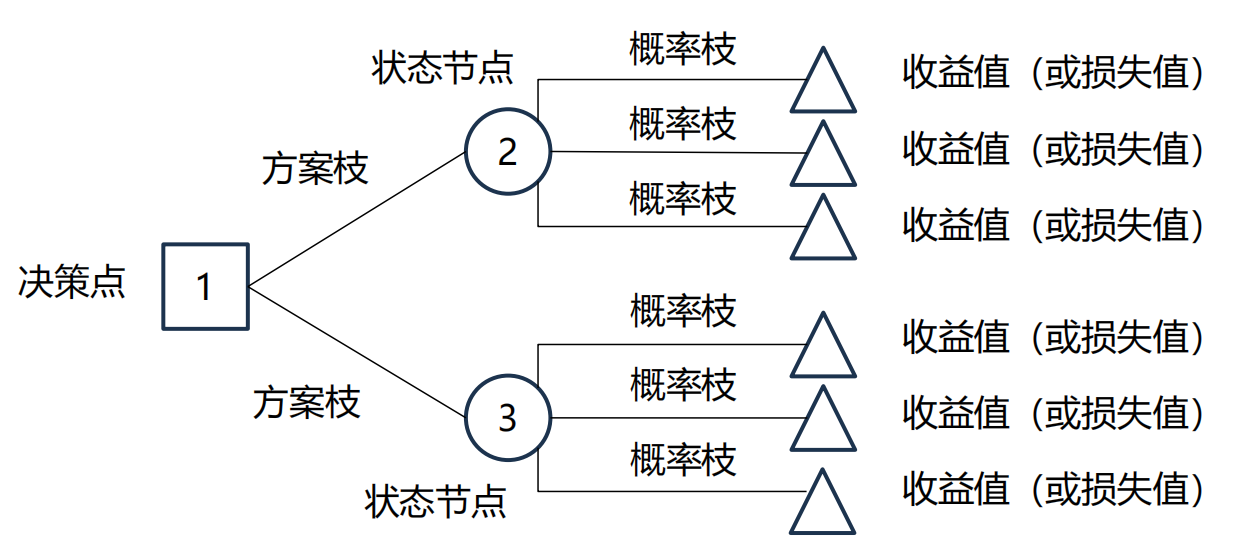
\includegraphics[width=10cm]{决策树.png}
\end{center}

决策点:以方框表示的节点,一般决策点位于决策树的最左端,即决策树的起点,如果属于多阶段决策问题,
决策树图形中可以有多个决策点,以决策树“根”部的决策点为最终决策方案。

方案枝:由决策点起自左向右画出的若干直线,每条方案枝代表一个备选的决策方案,代表备选方案的方案枝一般是两枝或者两枝以上。

状态节点:以圆圈表示的节点,位于每条方案枝的末端,状态节点是备选方案分支的终点,
也是每个备选方案可能遇到的自然状态的起点,一般将对应方案的期望损益值标记于用状态节点上方。

概率枝:从状态节点引出的若干条线,每条线代表一种自然状态及其可能出现的概率,每条分枝上面注明自然状态及其概率。

结果点:概率枝末端的三角节点,结果节点处列出不同的备选方案在相应的自然状态下的收益值或者损失值。

\noindent
\textbf{例:}

\begin{center}
    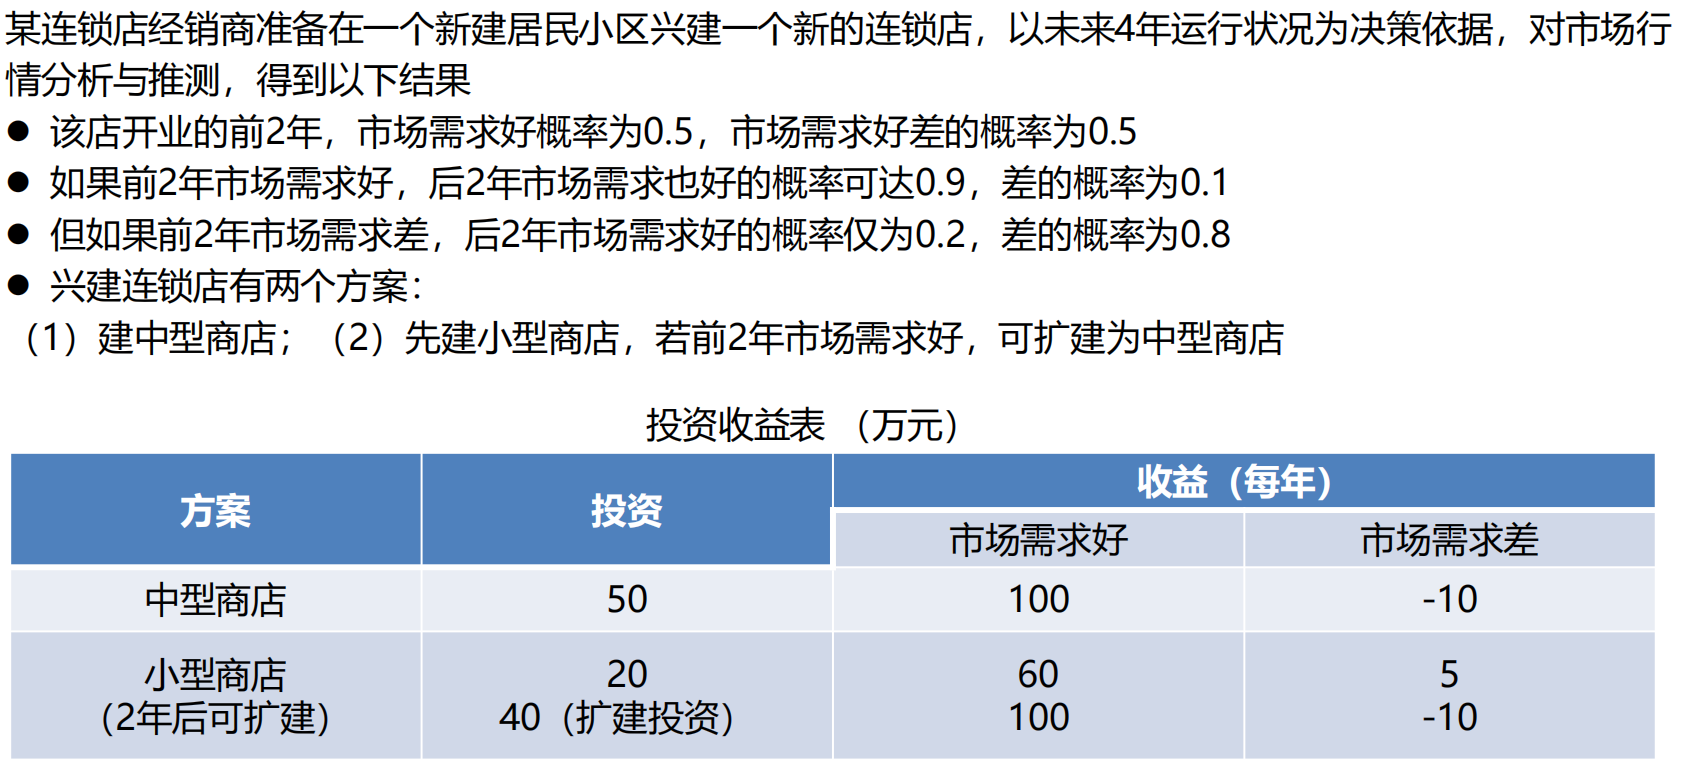
\includegraphics[width=10cm]{决策树例题目.png}
    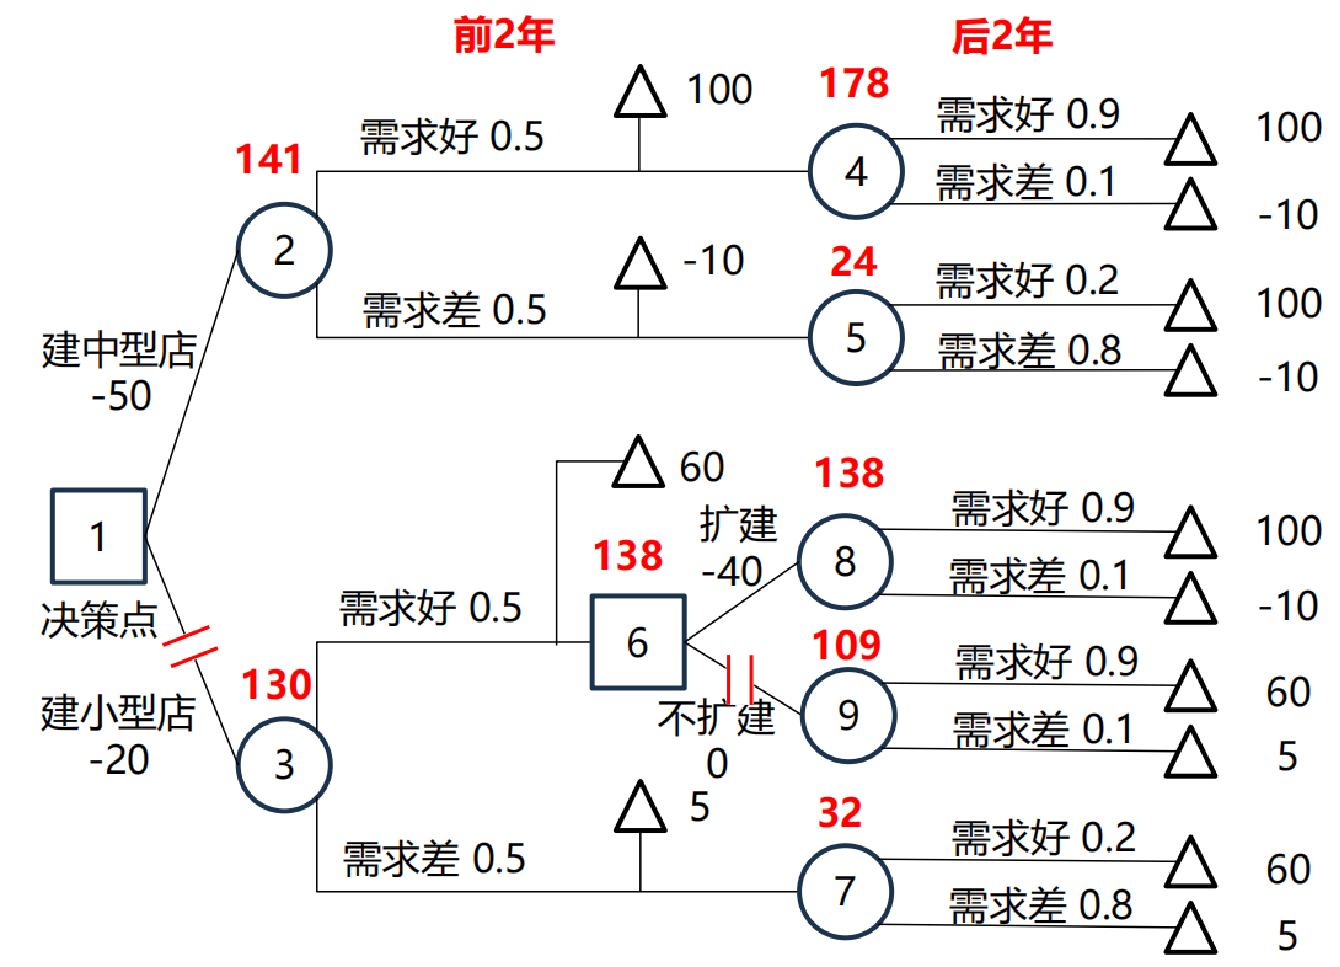
\includegraphics[width=10cm]{决策树例解答.png}
\end{center}

\subsection{贝叶斯决策的基本方法}

\noindent
\textbf{贝叶斯决策的问题}

设风险决策问题的自然状态为$s$,有$n$种离散的自然状态$s_i(i=1,2,\dots,n)$,
通过调查分析获得的补充信息用已发生的随机事件$E$表示,
信息值的可靠程度用随机事件$E$在自然状态$s$下发生的条件概率分布$P\left(E\mid s\right)$表示,
补充信息的随机事件有$m$种可能$E_j(j=1,2,\dots,m)$,则条件分布矩阵为
$$
\begin{bmatrix}P\left(E_1\mid s_1\right) & P\left(E_1\mid s_2\right) & \cdots & P\left(E_1\mid s_n\right) \\P\left(E_2\mid s_1\right) & P\left(E_2\mid s_2\right) & \cdots & P\left(E_2\mid s_n\right) \\\vdots & \vdots & \ddots & \vdots \\P\left(E_m\mid s_1\right) & P\left(E_m\mid s_2\right) & \cdots & P\left(E_m\mid s_n\right)\end{bmatrix}
$$
这个矩阵称为贝叶斯决策的似然分布矩阵。此矩阵完整描述了:在不同自然状态$s_i$条件下,调查分析信息$E_j$的可靠程度。


\noindent
\textbf{贝叶斯决策的基本步骤}

首先,根据似然分布矩阵,计算
$$
P\left(E_j\right)=\sum_{i=1}^nP\left(s_i\right)P\left(E_j\mid s_i\right)
$$
$$
P\left(s_i\mid E_j\right)=\frac{P\left(E_j\mid s_i\right)P\left(s_i\right)}{P\left(E_j\right)}
$$
在不同的调查结果$E_j$下,计算不同的决策方案$C_k$的收益期望
$$
E\left(C_k\right)=\sum_{i=1}^nP\left(s_i\mid E_j\right)c_{ki}
$$
其中$c_{ki}$为在决策方案$C_k$下出现自然状态$s_i$的收益,找到其中最大的期望值
$$
E\left(C_{opt}\mid E_j\right)=\max_kE\left(C_k\right)
$$
则经过调查后,期望收益为
$$
E\left(C_{opt}\right)=\sum_{j=1}^mE\left(C_{opt}\mid E_j\right)P\left(E_j\right)
$$

决策者在掌握补充信息$E_j$后,决策变化导致的期望收益的增量或期望损失的减少量称为补充信息$E_j$的价值:
$$
\text{EVAI}_{E_j}=E\left(C_{updated}\mid E_j\right)-E\left(C_{original}\mid E_j\right)
$$
全部补充信息$E_j$的价值的期望称为补充信息的价值:
$$
\text{EVAI}=E(\text{EVAI}_{E_j})
$$

也可以使用如下公式直接计算补充信息的价值
$$
\text{EVAI}=E\left(C_{posterior}\right)-E\left(C_{prior}\right)
$$

设补充信息为$E_j$,若存在自然状态$s_i$,使得条件概率$P\left(s_i\mid E_j\right)=1$,
当自然状态$s\ne s_i$时,总有$P\left(s\mid E_j\right)=0$,则称信息$E_j$为完全信息。

备选方案$a_k(k=1,2,\dots,m)$的决策结果(损益值)为随机变量$C_k$,
其在自然状态$s_i(i=1,2,\dots,n)$下的取值为$c_{ki}$ ,决策者在掌握完全信息$E_j$后($P\left(s_i\mid E_j\right)=1$),
决策变化导致的收益的增量或期望损失的减少量,称为完全信息$E_j$的价值
$$
\text{EVPI}_{E_j}=E\left(C_{updated}\mid E_j\right)-E\left(C_{original}\mid E_j\right)=\max_{1\le k\le m}(c_{ki})-c_{k_{original}i}
$$

如果全部补充信息价值的均为完全信息,则完全信息$E_j$价值的期望,
称为完全信息价值(Expected Value of Perfect Information, EVPI)
$$
\text{EVPI}=E\left(\text{EVPI}_{E_j}\right)
$$

实际上,完全信息可以看做条件分布矩阵为单位矩阵的补充信息,完全信息价值即为
$$
\text{EVPI}=\left[\sum_{i=0}^n\max_{1\le k \le m}(c_{ki})P(s_i)\right]-E\left(C_{original}\right)
$$

\subsection{效用理论及风险评价}

\noindent
\textbf{决策问题的表达}

对于一个决策问题,每一种备选方案(Decision Alternatives)对应不同的自然状态(States of Nature)
都有一个方案结果(Decision Outcomes),因此每一个决策方案的结果可以用一个向量表示。

评价各备选方案的优劣,需要将每个备选方案对应的向量映射为一个标量,对方案进行排序,
故决策分析的首要任务在于构建有效的映射方法或者模型。

\noindent
\textbf{事态体(Lottery)}

具有两种或两种以上可能结果的备选方案称为事态体,其中的各种可能结果为以一定概率出现的随机事件,如用$T$表示一个事态体,则
$$
T=\left(\theta_1,p_1;\theta_2,p_2;\dots;\theta_n,p_n\right)
$$
式中,$\theta_1,\theta_2,\dots,\theta_n$表示该方案在$n$种不同自然状态下的方案结果,
它们出现的概率分别为$p_1,p_2,\dots,p_n$,且满足$p_i\ge 0(i=1,2,\dots,n)$,$\sum_{i=1}^np_i=1$。

特别地,当$n=2$时,事态体$T=\left(\theta_1,p_1;\theta_2,p_2\right)$为简单事态体,
由于$p_1+p_2=1$,$p_2$可由$p_1$确定,故简单事态体可以简记为$T=\left(\theta_1,p_1;\theta_2\right)$。

若一个备选方案具有必然结果$x$,可记为$\left(x\right)$,它可以看作以概率$1$出现后果$x$的一个简单事态体,
即$\left(x\right)=\left(x,1;y\right)$,其中$y$为任意后果(通常可取为$0$),
也可以表示为具有相同结果的简单事态体$\left(x\right)=\left(x,p;x\right)$,其中$p$为任意概率。

风险型决策问题中,每一个备选方案$A_i$均可用一事态体表示,$p_j$为第$j$种自然状态出现的概率,
$\theta_{ij}$表示该备选方案在第$j$种自然状态出现时的后果。

全体事态体的集合$F$称为事态体空间,$F=\left\{T_1,T_2,\dots,T_n\right\}$。

事态体空间$F$中,所有可能后果的集合$J$称为后果集,$J=\left\{\theta_1,\theta_2,\dots,\theta_m\right\}$。

\noindent
\textbf{后果的偏好关系}

对于后果集$J=\left\{\theta_1,\theta_2,\dots,\theta_m\right\}$中任意两个可能的结果$x$和$y$,
总可以按照既定目标的需求,对二者的优劣进行排序:
\begin{itemize}[itemsep=0pt,parsep=0pt]
    \item $x$优于$y$,记为$x\succ y$
    \item $x$与$y$无差别,记为$x\sim y$
    \item $x$优于$y$或无差别于$y$,记为$x\succeq y$
\end{itemize}  

偏好关系满足以下三个条件:
\begin{itemize}[itemsep=0pt,parsep=0pt]
    \item 自反性:一个结果不会比自己差,即$x\succeq x$
    \item 传递性:$x\succeq y,y\succeq z \Rightarrow x\succeq z$
    \item 完备性:任何两个结果$x$和$y$都可以比较优劣,并且有两种情况之一:$x \succeq y$或$y\succeq x$
\end{itemize} 

\noindent
\textbf{事态体的偏好关系}

[假设1]简单事态体的偏好关系

设$T_1$和$T_2$是两个有相同可能结果的简单事态体,
即$T_1=\left(\theta_1,p;\theta_2\right)$,$T_2=\left(\theta_1,q;\theta_2\right)$,设$\theta_1 \succeq \theta_2$,则
\begin{itemize}[itemsep=0pt,parsep=0pt]
    \item 当$p=q$时,两个事态体之间无差别,记为$T_1 \sim T_2$
    \item 当$p>q$时,事态体$T_1$优于或者无差别于事态体$T_2$,记为$T_1\succeq T_2$
    \item 当$p<q$时,事态体$T_1$劣于或者无差别于事态体$T_2$,记为$T_1\preceq T_2$
\end{itemize} 

[假设2]连续性

设有两个简单事态体$T_1$和$T_2$,$T_1=\left(\theta_1,p;\eta\right)$,$T_2=\left(\theta_2,q;\eta\right)$,
设$\theta_1 \succeq \theta_2 \succeq \eta$,则
\begin{itemize}[itemsep=0pt,parsep=0pt]
    \item 当$p=q$时,$T_1 \succeq T_2$
    \item 存在$r\le q$,当$p=r$时,$T_1\sim T_2$
\end{itemize} 

[假设3]传递性

设$T_1$、$T_2$、$T_3$为三个事态体,则
\begin{itemize}[itemsep=0pt,parsep=0pt]
    \item 当$T_1\sim T_2$,$T_2\sim T_3$时,$T_1\sim T_3$
    \item 当$T_1 \succeq T_2$,$T_2 \succeq T_3$时,$T_1 \succeq T_3$
\end{itemize}

[定理1]无差性

设事态体$T_1=\left(\theta_1,x;\theta_2\right)$,事态体$T_2=\left(\theta_3\right)$为必然事件,
$\theta_1\succeq\theta_3\succeq\theta_2$,则必存在$p\in\left[0,1\right]$,使得当$x=p$时,
事态体$T_1$无差别于必然事件事态体$T_2$,即$\left(\theta_3\right)\sim\left(\theta_1,p;\theta_2\right)$,
此时称$p$为$\theta_3$关于$\theta_1,\theta_2$的无差概率,其随$\theta_3$变化:$\theta_3$越优,$p$越大。

设$p$为某一固定值,使得$\left(\theta_3\right)\sim\left(\theta_1,p;\theta_2\right)$的$\theta_3$后果称为等价确定值。

[定理2]简化性

任一有$n$种可能结果的事态体$T=\left(\theta_1,p_1;\theta_2,p_2;\cdots;\theta_n,p_n\right)$,
无差于某一简单事态体$T_2=\left(\theta^*,p;\theta_*\right)$,即
$$
\left(\theta_1,p_1;\theta_2,p_2;\cdots;\theta_n,p_n\right)\sim\left(\theta^*,p;\theta_*\right)
$$
其中$\theta^*\succeq\max_j\left(\theta_j\right),\theta_*\preceq\min_j\left(\theta_j\right)$,
$p=\sum_{j=1}^np_jq_j$,$q_j$为$\theta_j$关于$\theta^*$与$\theta_*$的无差概率。

[不同备选方案的比较]风险决策问题中,每个备选方案都构成一个事态体,对于备选方案集合$A=\left\{A_1,A_2,\cdots,A_m\right\}$,有
$$
A_i=\left(\theta_{i1},p_1;\theta_{i2},p_2;\cdots;\theta_{in},p_n\right)\kern 36pt i=1,2,\cdots,m
$$
$$
A_i\sim \left(\theta^*,\sum_{j=1}^np_jq_{ij};\theta_*\right)\kern 36pt
\theta^*\succeq\max_{i,j}\left(\theta_{ij}\right),\theta_*\preceq\min_{i,j}\left(\theta_{ij}\right)
$$
$$
\left(\theta_{ij}\right)\sim\left(\theta^*,q_{ij};\theta_*\right)\kern 36pt i=1,2,\cdots,m;j=1,2,\cdots,n
$$
通过比较$\sum_{j=1}^np_jq_{ij}(i=1,2,\cdots,m)$之间的大小,即可对备选方案进行排序,其值越大,方案越优。

\noindent
\textbf{效用}

$q_{ij}$可以视为以$\theta_{ij}$为自变量、值域为实数区间$\left[0,1\right]$的函数,即$q_{ij}=u\left(\theta_{ij}\right)$。
$\theta_{ij}$的优劣,本质是该后果对决策主体所能提供的作用或者价值大小,称其为对决策主体的效用(Utility)。
$q_{ij}$成为衡量效用大小的值,称为效用值,$u\left(\theta_{ij}\right)$称为效用函数。

备选方案$A_i$的期望效用值为:
$$
E\left(A_i\right)=\sum_{j=1}^np_jq_{ij}=\sum_{j=1}^np_j\cdot u\left(\theta_{ij}\right)
$$

\noindent
\textbf{效用函数}

对于一个决策问题,所有方案后果的集合为$J=\left\{\theta_1,\theta_2,\dots,\theta_m\right\}$,
取$\theta^*\succeq\max_j\left(\theta_j\right),\theta_*\preceq\min_j\left(\theta_j\right)$,
若定义在集$\Theta=\left\{x\mid\theta^*\succeq x\succeq\theta_*\right\}$上的实值函数$u\left(x\right)$满足:
\begin{enumerate}[itemsep=0pt,parsep=0pt]
    \item 单调性:$u\left(a\right)\ge u\left(b\right)\Leftrightarrow a\succeq b$,
    $u\left(a\right)=u\left(b\right)\Leftrightarrow a\sim b$
    \item $u\left(\theta^*\right)=1$,$u\left(\theta_*\right)=0$
    \item 若$\left(c\right)\sim\left(a,p;b\right)$,
    则$u\left(c\right)=p\cdot u\left(a\right)+(1-p)\cdot u\left(b\right)$,其中$a,b,c\in\Theta$
\end{enumerate} 
则称函数$u\left(x\right)$为效用函数。

特别的,取$a=\theta^*,b=\theta_*$时,若$\left(\theta\right)\sim\left(\theta^*,p;\theta_*\right)$,
则$u\left(\theta\right)=p\cdot u\left(\theta^*\right)+(1-p)\cdot u\left(\theta_*\right)=p$。

确定某一决策者的效用曲线的步骤:
\begin{enumerate}[itemsep=0pt,parsep=0pt]
    \item 确定最大收益效用值和最小收益效用值$u\left(\theta^*\right)=1$,$u\left(\theta_*\right)=0$
    \item 根据两组已定的结果与效用值$a,u\left(a\right),b,u\left(b\right)$,调整直接获得的收益,做出选择,
    直至两种方案对决策者无差别,即找到使$u\left(x\right)=\frac{1}{2}\left[u\left(a\right)+u\left(b\right)\right]$的$x$值。
    重复该步骤以使效用曲线更完整。
\end{enumerate} 
  
效用曲线有以下四种类型:
\begin{itemize}[itemsep=0pt,parsep=0pt]
    \item 风险中性型:决策者对风险持中立态度,可以直接用方案结果决策。
    \item 风险厌恶型:决策者对利益的反应比较迟缓(斜率小),而对损失的反应敏感(斜率大),要规避风险,曲线呈上凸形状。
    \item 风险偏好型: 决策者想获得更大利益,而不关心损失,对利益的反应比较敏感,而对损失的反应迟缓,曲线呈下凹形状。
    \item 渴望型: 在结果值偏低,或者存在损失时,呈现风险偏好(放手一搏),而在收益到达一定程度后,转为稳妥策略。
\end{itemize}

\begin{center}
    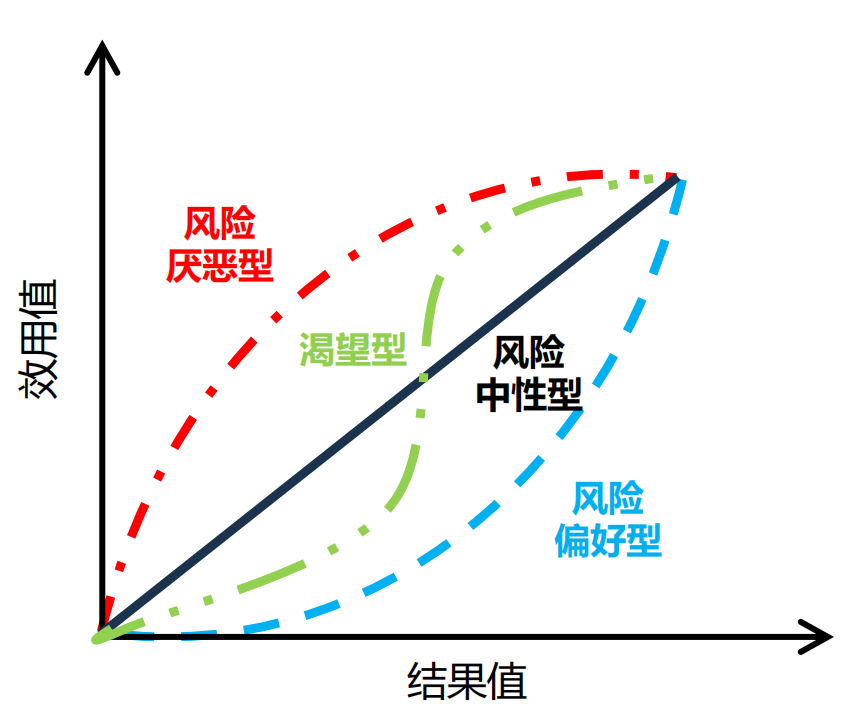
\includegraphics[width=10cm]{效用函数类型.png}
\end{center}

\section{单目标决策——不确定型决策}

不确定型决策是指完全不掌握自然状态出现概率的决策。

\subsection{不确定型决策的决策准则}

\noindent
\textbf{悲观准则}

决策者考虑由于决策失误可能造成的重大损失,设想采取任何一个方案都是收益最小的状态发生,
从最小收益值中选择最大方案,这一准则也称为最小最大准则。即
$$
C_{min}\left(a\right)=\min_{s\in S}C\left(a,s\right)
$$
$$
a^*=\text{arg}\max_{a\in A}C_{min}\left(a\right)
$$

\noindent
\textbf{乐观准则}
 
决策者不会放弃任何一个可以获得最好结果的机会,设想采取任何一个方案都是收益最大的状态发生,
从最大收益值中选择最大方案,这一准则也称为最大最大准则。即
$$
C_{max}\left(a\right)=\max_{s\in S}C\left(a,s\right)$$
$$
a^*=\text{arg}\max_{a\in A}C_{max}\left(a\right)
$$

\noindent
\textbf{折中准则}
 
决策者既不过于乐观,也不过于悲观,采用一种折中态度:设乐观系数$\alpha(0\le\alpha\le 1)$,则
$$
C_{mid}\left(a\right)=\alpha\cdot\max_{s\in S}C\left(a,s\right)+\left(1-\alpha\right)\cdot\min_{s\in S}C\left(a,s\right)
$$
$$
a^*=\text{arg}\max_{a\in A}C_{mid}\left(a\right)
$$
其中:乐观系数为$1$时,对应乐观决策;乐观系数为$0$时,对应悲观决策。

\noindent
\textbf{后悔值准则}

决策者所选的备选方案不是在实际出现的自然状态下的最好方案,便会感到后悔:
后悔值定义为所选方案的收益与实际出现自然状态下的最优方案收益之差,通过最小化每种备选方案的最大后悔值,进行决策。即
$$
C_r\left(a,s\right)=\max_{a_i\in A}\left(C\left(a_i,s\right)\right)-C\left(a,s\right)
$$
$$
C_r\left(a\right)=\max_{s\in S}C_r\left(a,s\right)
$$
$$
a^*=\text{arg}\min_{a\in A}C_r\left(a\right)
$$

\noindent
\textbf{等概率准则}

将$n$种自然状态出现的概率假设为相等,均为$\frac{1}{n}$,通过计算期望收益进行决策。即
$$
C_{eq}=\frac{\sum_{j=1}^nC_{ij}}{n}
$$
$$
a^*=\text{arg}\max_{a\in A}C_{eq}\left(a\right)
$$

\section{多目标决策}

\subsection{多目标决策问题的基本概念}

\noindent
\textbf{多目标问题的解集}

对于$m$个目标,一般用$m$个目标函数$f_1(x),f_2(x),\cdots,f_m(x)$表示,其中$x$表示备选方案。解的分类如下:
\begin{itemize}[itemsep=0pt,parsep=0pt]
    \item 劣解:方案$A$的各自目标均劣于另一方案$B$的各目标,则方案$A$可以直接舍去,这样的方案$A$称为劣解。
    \item 非劣解:既不能立即舍去,也不能立即定为最优的方案称为非劣解,在多目标决策中起着非常重要的作用。
    \item 最优解:在所有的目标上均不比其他方案差的解称为最优解。设最优解为$x^*$,则其满足$f_i(x^*)\ge f_i(x),i=1,2,\cdots,m$。
    \item 选好解:若无最优解,则从备选方案中找出所有非劣解,然后权衡非劣解,从中找出一个比较满意的方案。
\end{itemize}

\noindent
\textbf{决策矩阵}
 
要从现有的$n$个备选方案$A_1,A_2,\cdots,A_n$中选取最优方案,
决策者决策时需要考虑的目标有$m$个,$G_1,G_2,\cdots,G_m$,决策者可以通过调查评估获得以下信息:
\begin{center}
    \begin{tabular}{|c|c|c|c|c|}
        \hline
                 & $G_1$    & $G_2$    & $\cdots$ & $G_m$    \\ \hline
        $A_1$    & $a_{11}$ & $a_{12}$ & $\cdots$ & $a_{1m}$ \\ \hline
        $A_2$    & $a_{21}$ & $a_{22}$ & $\cdots$ & $a_{2m}$ \\ \hline
        $\vdots$ & $\vdots$ & $\vdots$ & $\ddots$ & $\vdots$ \\ \hline
        $A_n$    & $a_{n1}$ & $a_{n2}$ & $\cdots$ & $a_{nm}$ \\ \hline
    \end{tabular}
\end{center}
其中$a_{ij}$表示第$i$个方案第$j$个目标的后果值,该表格可以用矩阵形式表示:
$$
\begin{bmatrix}a_{11} & a_{12} & \cdots & a_{1m} \\
    a_{21} & a_{22} & \cdots & a_{2m} \\
    \vdots & \vdots & \ddots & \vdots \\
    a_{n1} & a_{n2} & \cdots & a_{nm}
\end{bmatrix}
$$
该矩阵称为决策矩阵,是大多数决策分析方法的基础。

\noindent
\textbf{目标的权重}

多目标决策过程中,决策者所考虑的多个目标对决策的重要程度并不是相同的,存在相对差别,通常通过赋予各目标一定的权重进行决策,
以权重表示各目标的重要程度,权重越大,对应的目标越重要。在已知各目标的权重后,决策准则为:
$$
E\left(A_i\right)=\sum_{j=1}^m\lambda_ja_{ij}
$$
其中$\lambda_j$为第$j$个目标的权重。

附:记决策矩阵为$A$,$\overrightarrow E=\begin{bmatrix}E(A_1) & E(A_2) & \cdots & E(A_n)\end{bmatrix}^T$,
$\overrightarrow \Lambda=\begin{bmatrix}\lambda_1 & \lambda_2 & \cdots & \lambda_m\end{bmatrix}^T$,
则$\overrightarrow E=A\overrightarrow\Lambda$。

\subsection{层次分析法}

运用层次分析法构造系统模型时,大体可以分为以下四个步骤:

\noindent
\textbf{1. 多级递阶结构}

将决策问题分为3个或多个层次:
\begin{enumerate}[itemsep=0pt,parsep=0pt]
    \item 最高层:目标层。表示解决问题的目的,即层次分析要达到的总目标;通常只有一个总目标。
    \item 中间层:准则层 。表示采取某种措施、政策、方案等实现预定总目标所涉及的中间环节。
    \item 最低层:方案层(指标层)。表示将选用的解决问题的各种措施、政策、方案等;通常有几个方案可选。
\end{enumerate} 
每层有若干元素,层间元素的关系用相连直线表示。

根据层与层之间的联系情况,层次结构可以分为三种:
\begin{itemize}[itemsep=0pt,parsep=0pt]
    \item 完全相关结构:上一层的每一个要素与下一次的所有要素均有联系。
    \begin{center}
        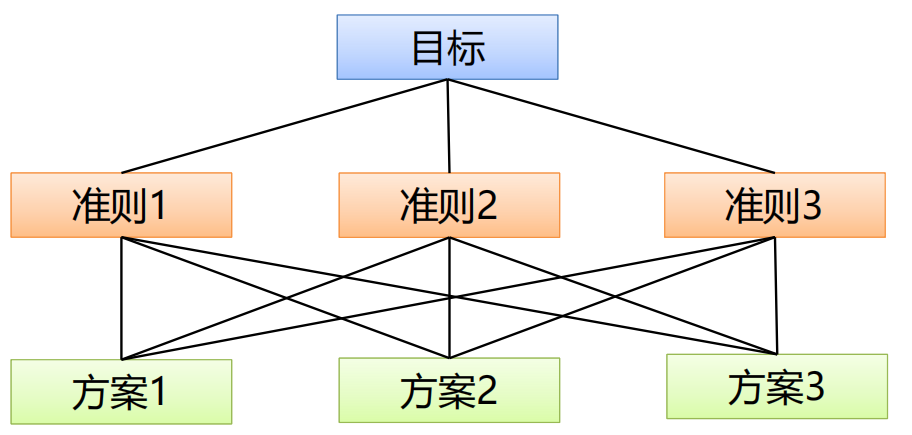
\includegraphics[width=10cm]{完全相关结构.png}
    \end{center}
    \item 完全独立性结构:上一层的每一个要素都有各自独立的、完全不相同的下层要素。
    \begin{center}
        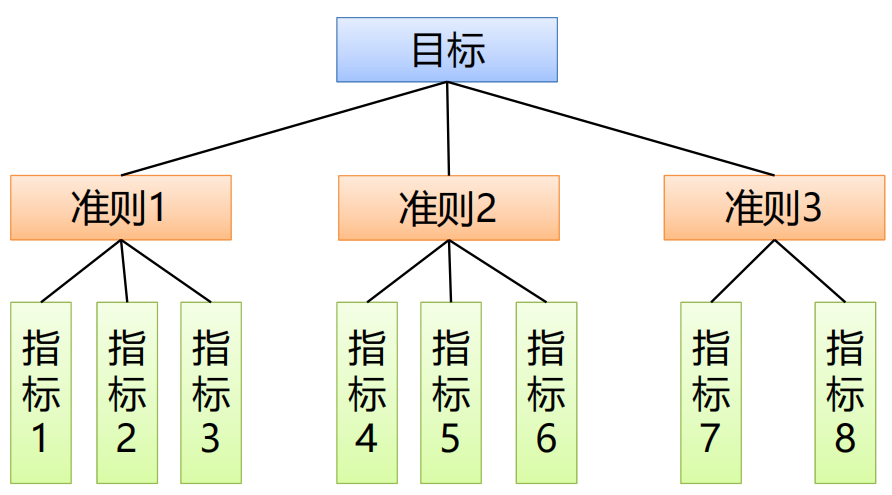
\includegraphics[width=10cm]{完全独立性结构.png}
    \end{center}
    \item 混合结构:由上述两种结构结合的混合结构。
    \begin{center}
        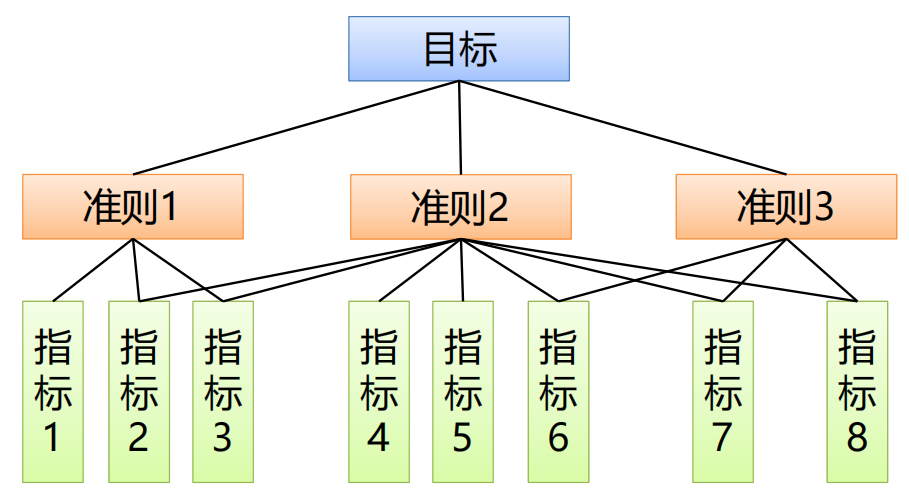
\includegraphics[width=10cm]{混合结构.png}
    \end{center}
\end{itemize}

\noindent
\textbf{2. 判断矩阵}

判断矩阵也称为成对比较矩阵,是表示本层所有因素针对上一层某一个因素的相对重要性的比较。
(心理学家认为成对比较的因素不宜超过9个,即每层不要超过9个因素)

设对于目标$A$或者准则$C$,其下一层具有$n$个要素$E_1,E_2,\dots,E_n$。以上一层的要素作为判断标准,
对下一层的$n$个要素进行两两比较,确定判断矩阵的元素值。判断矩阵中的$a_{ij}$,
表示以准则$C$的角度考虑要素$E_i$对$E_j$的相对重要程度。

若假设在准则$C$下,要素$E_1,E_2,\dots,E_n$的权重分别为$w_1,w_2,\dots,w_n$,
即权重向量$\overrightarrow W=\begin{bmatrix} w_1 & w_2 & \cdots & w_n\end{bmatrix}^T$,
则$a_{ij}=\frac{w_i}{w_j}$,判断矩阵为
$$
A=\left(a_{ij}\right)_{n\times n}=\left(\frac{w_i}{w_j}\right)_{n\times n}=
\begin{bmatrix}
    \frac{w_1}{w_1} & \frac{w_1}{w_2} & \cdots & \frac{w_1}{w_n} \\
    \frac{w_2}{w_1} & \frac{w_2}{w_2} & \cdots & \frac{w_2}{w_n} \\
    \vdots          & \vdots          & \ddots & \vdots          \\
    \frac{w_n}{w_1} & \frac{w_n}{w_2} & \cdots & \frac{w_n}{w_n}
\end{bmatrix}
$$

易知在判断矩阵$A$满足:$a_{ij}>0$,$a_{ii}=1$,$a_{ij}a_{ji}=1$,称满足以上三个条件的方阵为正互反矩阵。
在实际问题中,一般是先得到判断矩阵$A$,再求得权重向量$\overrightarrow W$,在填写时$A$实际上只需要完成严格上三角矩阵部分。

判断矩阵中的元素$a_{ij}$是表示两个要素的相对重要性的数量尺度,称为判断尺度。
Saaty等人提出$1-9$尺度——$a_{ij}$取值$1,2,\dots,9$及其倒数$1,\frac12,\dots,\frac19$,
为了便于定性到定量的转化,设定了判断尺度的取值(倒数表示重要性相反):
\begin{center}
    \begin{tabular}{|c|c|}
        \hline
        $a_{ij}$尺度 & $E_i$相对于$E_j$的重要性 \\ \hline
        1 & $E_i$和$E_j$同样重要 \\ \hline
        2 & $\vdots$ \\ \hline
        3 & $E_i$比$E_j$稍微重要 \\ \hline
        4 & $\vdots$ \\ \hline
        5 & $E_i$比$E_j$重要 \\ \hline
        6 & $\vdots$ \\ \hline
        7 & $E_i$比$E_j$重要得多 \\ \hline
        8 & $\vdots$ \\ \hline
        9 & $E_i$比$E_j$绝对重要 \\ \hline
    \end{tabular}
\end{center}

当方阵$A$的元素$a_{ij}$满足$a_{ij}=\frac{a_{ik}}{a_{jk}}$时,称矩阵具有完全一致性,此时$A$的元素具有传递性。
具有完全一致性的判断矩阵$A=\left(\frac{w_i}{w_j}\right)_{n\times n}$的秩$\text{rank}=1$,
其只有一个非零特征值$n$,对应的特征向量为$\overrightarrow W$,即
$$
\begin{bmatrix}\frac{w_1}{w_1} & \frac{w_1}{w_2} & \cdots & \frac{w_1}{w_n} \\\frac{w_2}{w_1} & \frac{w_2}{w_2} & \cdots & \frac{w_2}{w_n} \\\vdots & \vdots & \ddots & \vdots \\\frac{w_n}{w_1} & \frac{w_n}{w_2} & \cdots & \frac{w_n}{w_n} \end{bmatrix}\begin{bmatrix}w_1 \\w_2 \\\vdots \\w_n\end{bmatrix}=n\begin{bmatrix}w_1 \\w_2 \\\vdots \\w_n\end{bmatrix}
$$

\noindent
\textbf{3. 相对重要度}
 
特征根法:判断矩阵$A$的最大特征值所对应的特征向量即为权重向量$\overrightarrow W$。

可先求出判断矩阵最大特征值对应的特征向量,再经过归一化处理,即可得到要素关于准则的权重,即相对重要度。

\noindent
\textbf{4. 相容性判断}

定理: $n$阶正互反阵$A$的最大特征值$\lambda_{max}\ge n$,且$\lambda_{max}=n$时$A$为一致阵。

当判断矩阵大于$3$阶时,增加了比较判断的复杂度,可能出现出现甲比乙极端重要,乙比丙极端重要,
而丙又比甲极端重要的判断,一般是违反常识的,这样会使得一致性不能被满足。

\begin{itemize}[itemsep=0pt,parsep=0pt]
    \item 当判断矩阵最大特征值$\lambda_{max}=n$时,称其为完全相容判断矩阵;
    \item 当判断矩阵最大特征值$\lambda_{max}>n$时,所建立的判断矩阵有偏差,称为不相容判断矩阵。
\end{itemize}

一般地,我们并不严格要求判断具有这种传递性和一致性,这是由客观事物的复杂性与人认识的多样性所决定的。
但在构造两两判断矩阵时,要求判断是近似一致的。当判断矩阵过于偏离一致性时,用上述各种方法计算的排序权重作为决策依据,
其可靠程度也值得怀疑,可能导致决策的失误,因而必须对判断矩阵的一致性进行检验。

定义一致性指标(Consistence Index)
$$
\text{CI}=\frac{\lambda_{max}-n}{n-1}
$$
其含义为判断矩阵$A$除最大特征值外的所有特征值的平均值。
当$\text{CI}=0$时,$A$具有完全一致性;$\text{CI}$越接近$0$,$A$具有越强的一致性;$\text{CI}$越大,不一致性越严重。

判断矩阵的维数$n$越大,判断的一致性将越差,故一般放宽对高维判断矩阵一致性的要求。
引入修正值$\text{RI}$,其本质是完全随机的$\text{CI}$的期望,即$\text{RI}=E\left(\text{CI}\right)$,其参考表格如下:
\begin{center}
    \begin{tabular}{|c|c|c|c|c|c|c|c|c|}
        \hline
        阶数        & 1    & 2    & 3    & 4    & 5    & 6    & 7    & 8    \\ \hline
        $\text{RI}$ & /    & /    & 0.52 & 0.89 & 1.12 & 1.26 & 1.36 & 1.41 \\ \hline
        阶数        & 9    & 10   & 11   & 12   & 13   & 14   & 15   &      \\ \hline
        $\text{RI}$ & 1.46 & 1.49 & 1.52 & 1.54 & 1.56 & 1.58 & 1.59 &      \\ \hline
    \end{tabular}
\end{center}

利用一致性比率$\text{CR}=\frac{\text{CI}}{\text{RI}}$作为衡量判断矩阵一致性的指标,
当$\text{CR}\le0.10$时,可认为判断矩阵具有相容性,据此计算的权重向量是可以接受的,否则需要重新进行两两比较判断。

\noindent
\textbf{层次分析法综合应用过程}

对于含目标层、准则层、方案层三个层次的决策问题,层次分析法过程如下:

假设有1个总目标$O$,$m$个准则$C_1,C_2,\dots,C_m$,$n$个方案$P_1,P_2,\dots,P_n$,各层之间为全连接。
\begin{enumerate}[itemsep=0pt,parsep=0pt]
    \item 根据判断尺度写出所有的判断矩阵(一共$1+m$个方阵,其中$1$个$m$阶,$m$个$n$阶)。
    \item 求出每个判断矩阵的最大特征值$\lambda_{max}$,并判断其是否通过一致性检验,若是,则继续,
    若否,重新进行两两比较判断得到新的判断矩阵。
    \item 求出每个判断矩阵的最大特征值对应的特征向量,并做归一化得到$\overrightarrow W$。
    \item 记准则层对目标的判断矩阵对应的权重向量为
    $\overrightarrow {W_c}=\begin{bmatrix}c_1 & c_2 & \cdots & c_m\end{bmatrix}^T$,
    方案层对准则$C_j$的判断矩阵对应的权重向量为
    $\overrightarrow {W_j}=\begin{bmatrix}p_{1j} & p_{2j} & \cdots & p_{nj}\end{bmatrix}^T$,
    则方案$P_i$对目标的权值为$p_i=\sum_{j=1}^mc_jp_{ij}$。

    附:记$\overrightarrow P=\begin{bmatrix}p_1 & p_2 & \cdots & p_n\end{bmatrix}^T$,
    $W=\begin{bmatrix}\overrightarrow{W_1} & \overrightarrow{W_2} & \cdots & \overrightarrow{W_m}\end{bmatrix}$
    则$\overrightarrow P=W\overrightarrow{W_c}$
    \item 比较各个方案对目标的权值,选取最优方案。
\end{enumerate} 

\end{document}